\section{Análisis Exploratorio de Datos}

Haremos un análisis exploratorio para conocer el dataset en profundidad y poder identificar patrones, tendencias y relaciones entre las variables.
Esto nos permitirá tomar decisiones informadas sobre cómo abordar el problema de la incidencia delictiva más adelante en el proyecto,
principalmente para crear el modelo de predicción adecuado a este problema.

Para esto, haremos limpieza, análisis estadístico, detección de outliers y visualización de los datos.

Como mencionamos en la sección anterior, cada sección de este análisis se irá documentando con código y resultados, para pode seguir el
proceso de manera clara y transparente. De igual manera, el cuaderno de Jupyter con el código completo de este análisis se encuentra disponible
\href{https://github.com/wallsified/proyecto-final-aymdd/blob/yoba/modelo/notebooks/eda.ipynb}{aquí}, mientras que el código fuente de ésta
sección se encuentra disponible en \href{https://github.com/wallsified/proyecto-final-aymdd/tree/main/src/eda}{ésta carpeta} del repositorio
del proyecto.

\subsection{Diccionario de Datos}

\begin{lstlisting}[language=Python, caption={Código para generar el diccionario de datos}, label={lst:diccionario-datos}]
import sys
from pathlib import Path

# Resuelve el problema de las ubicaciones de los scripts
sys.path.insert(0, str(Path.cwd().parent))

import pandas as pd
import matplotlib.pyplot as plt
import seaborn as sns

from src import config
from src.data import DataRepository
from src.preprocessing import PreprocessingPipeline
from src.eda import StatisticsAnalyzer, OutlierDetector

# Tema visual por defecto del proyecto.
sns.set_theme(style=config.SEABORN_THEME, palette=config.PLOT_PALETTE)
pd.set_option("display.max_columns", 20)
pd.set_option("display.width", 140)
pd.set_option("display.max_colwidth", 200)

repo = DataRepository()
dataframe = repo.load()
repo.dictionary()
\end{lstlisting}

\begin{table}[ht]
  \centering
  \caption{Diccionario de datos}
  \small
  \resizebox{\textwidth}{!}{%
    \begin{tabular}{r l p{0.65\textwidth}}
      \hline
      \textbf{Índice} & \textbf{Nombre (tipo)} & \textbf{Descripción} \\
      \hline
      0 & \texttt{anio} (int64) & Año de registro de las averiguaciones previas y/o carpetas de investigación. \\
      1 & \texttt{clave\_ent} (int64) & Clave de la entidad, según el Marco Geoestadístico Nacional (MGN) del Instituto Nacional de Geografía y Estadística (INEGI). \\
      2 & \texttt{entidad} (str) & Entidad federativa de registro de las averiguaciones previas y/o carpetas de investigación. \\
      3 & \texttt{bien\_juridico\_afectado} (str) & Primera clasificación de los delitos en las averiguaciones previas y/o carpetas de investigación. (Patrimonio, vida, libertad, etc.) \\
      4 & \texttt{tipo\_delito} (str) & Segunda clasificación de los delitos. (Falsedad, Lesiones, Robo, etc.) \\
      5 & \texttt{subtipo\_delito} (str) & Tercera clasificación de los delitos. Subcategorías específicas de cada tipo de delito. (Lesiones dolosas, etc.). \\
      6 & \texttt{modalidad} (str) & Cuarta clasificación de los delitos. Forma en la que se comete el delito. (Con violencia, sin violencia, etc.) \\
      7 & \texttt{mes} (str) & Mes de registro de las averiguaciones previas y/o carpetas de investigación. \\
      8 & \texttt{fecha} (str) & Fecha de registro de las averiguaciones previas y/o carpetas de investigación. \\
      9 & \texttt{incidencia\_delictiva} (int64) & Incidencia delictiva del Fuero Común (Número absoluto de presuntos delitos registrados). \\
      10 & \texttt{entidad\_federativa} (str) & Entidad federativa de registro de las averiguaciones previas y/o carpetas de investigación. \\
      \hline
    \end{tabular}%
  }
  \label{tab:diccionario-datos}
\end{table}

\subsection{Overview del Dataset}

\begin{lstlisting}[language=Python, caption={Código para obtener un overview del dataset}, label={lst:overview-dataset}]
	dataframe
\end{lstlisting}

\begin{table}[ht]
  \centering
  \caption{Muestra del dataset: primeras filas}
  \scriptsize
  \resizebox{\textwidth}{!}{%
    \begin{tabular}{r r r l p{3.5cm} p{3cm} p{3cm} p{2.5cm} l l r l}
      \hline
      \textbf{idx} & \textbf{anio} & \textbf{clave\_ent} & \textbf{entidad} & \textbf{bien\_juridico\_afectado} & \textbf{tipo\_delito} & \textbf{subtipo\_delito} & \textbf{modalidad} & \textbf{mes} & \textbf{fecha} & \textbf{incidencia\_delictiva} & \textbf{entidad\_federativa} \\
      \hline
      0 & 2015 & 1 & Aguascalientes & El patrimonio & Abuso de confianza & Abuso de confianza & Abuso de confianza & Abril & 2015-04-01 & 22 & Aguascalientes \\
      1 & 2015 & 1 & Aguascalientes & El patrimonio & Abuso de confianza & Abuso de confianza & Abuso de confianza & Agosto & 2015-08-01 & 40 & Aguascalientes \\
      2 & 2015 & 1 & Aguascalientes & El patrimonio & Abuso de confianza & Abuso de confianza & Abuso de confianza & Diciembre & 2015-12-01 & 26 & Aguascalientes \\
      3 & 2015 & 1 & Aguascalientes & El patrimonio & Abuso de confianza & Abuso de confianza & Abuso de confianza & Enero & 2015-01-01 & 41 & Aguascalientes \\
      4 & 2015 & 1 & Aguascalientes & El patrimonio & Abuso de confianza & Abuso de confianza & Abuso de confianza & Febrero & 2015-02-01 & 33 & Aguascalientes \\
      \hline
    \end{tabular}%
  }
  \label{tab:dataset-head}
\end{table}

\begin{table}[ht]
  \centering
  \caption{Muestra del dataset: últimas filas}
  \scriptsize
  \resizebox{\textwidth}{!}{%
    \begin{tabular}{r r r l p{3.5cm} p{3cm} p{3cm} p{2.5cm} l l r l}
      \hline
      \textbf{idx} & \textbf{anio} & \textbf{clave\_ent} & \textbf{entidad} & \textbf{bien\_juridico\_afectado} & \textbf{tipo\_delito} & \textbf{subtipo\_delito} & \textbf{modalidad} & \textbf{mes} & \textbf{fecha} & \textbf{incidencia\_delictiva} & \textbf{entidad\_federativa} \\
      \hline
      413947 & 2025 & 32 & Zacatecas & Otros bienes jurídicos afectados (del fuero común) & Otros delitos del Fuero Común & Otros delitos del Fuero Común & Otros delitos del Fuero Común & Marzo & 2025-03-01 & 184 & Zacatecas \\
      413948 & 2025 & 32 & Zacatecas & Otros bienes jurídicos afectados (del fuero común) & Otros delitos del Fuero Común & Otros delitos del Fuero Común & Otros delitos del Fuero Común & Mayo & 2025-05-01 & 98 & Zacatecas \\
      413949 & 2025 & 32 & Zacatecas & Otros bienes jurídicos afectados (del fuero común) & Otros delitos del Fuero Común & Otros delitos del Fuero Común & Otros delitos del Fuero Común & Noviembre & 2025-11-01 & 92 & Zacatecas \\
      413950 & 2025 & 32 & Zacatecas & Otros bienes jurídicos afectados (del fuero común) & Otros delitos del Fuero Común & Otros delitos del Fuero Común & Otros delitos del Fuero Común & Octubre & 2025-10-01 & 99 & Zacatecas \\
      413951 & 2025 & 32 & Zacatecas & Otros bienes jurídicos afectados (del fuero común) & Otros delitos del Fuero Común & Otros delitos del Fuero Común & Otros delitos del Fuero Común & Septiembre & 2025-09-01 & 133 & Zacatecas \\
      \hline
    \end{tabular}%
  }
  \label{tab:dataset-tail}
\end{table}

El dataset contiene 413,952 registros que abarcan desde enero de 2015 hasta diciembre de 2025 (11 años).
Los datos están organizados a nivel estatal con granularidad mensual (32 entidades × 40+ tipos de delito × 132 meses),
lo que nos permite hacer análisis longitudinales de la evolución del delito en cada estado.

\subsection{Calidad y Limpieza de los Datos}

Haremos lo siguiente con el dataset original:

\begin{itemize}
  \item Borramos las columnas \texttt{anio} y \texttt{mes} para poder trabajar únicamente con fecha. Posteriormente, ésta última pasará a ser de tipo \texttt{datetime}.
  \item \texttt{entidad\_federativa} es un duplicado de \texttt{entidad}, por lo que borramos ésta columna.
  \item \texttt{clave\_entidad} no nos es de utilidad al ya tener el nombre de las entidades, por lo que borramos ésta columna.
  \item Analizamos el dataset en busca de duplicados y valores nulos.
  \item Consideraremos que una entrada es inválida si tiene valores NaN en \texttt{incidencia\_delictiva}, \texttt{fecha} y \texttt{entidad}. Una vez detectadas, serán eliminadas.
  \item Por revisión manual, vemos que algunos estados tienen su nombre completo, como \texttt{Veracruz de Ignacio de la Llave}. Acortaremos el nombre de estos estados para una visualización más limpia de la información.
\end{itemize}

\begin{lstlisting}[language=Python, caption={Código para limpiar el dataset}, label={lst:limpieza-dataset}]
cleaning_pipeline = PreprocessingPipeline(
    drop_columns=["anio", "clave_ent", "mes", "entidad_federativa"]
)
clean_dataset = cleaning_pipeline.run(dataframe)
# reorganizamos las columnas para tener la fecha como columna inicial del dataset
clean_dataset = clean_dataset.iloc[:, [5, 0, 1, 2, 3, 4, 6]]
cleaning_pipeline.save(clean_dataset)
\end{lstlisting}

\begin{lstlisting}
[1] Eliminando columnas declaradas en drop_columns
 Eliminadas: ['anio', 'clave_ent', 'mes', 'entidad_federativa']
[2] Convirtiendo '{self._date_col}' a datetime
   OK=413,952 / fallidos=0
 Rango: 2015-01-01 - 2025-12-01
[3] Eliminando filas con nulos en críticas
Filas: 413,952 - 413,952 (eliminadas: 0)
[4] Eliminando duplicados exactos
Filas: 413,952 - 413,952 (eliminadas: 0)
[5] Normalizando nombres de entidades federativas
413,952 filas x 7 columnas,
\end{lstlisting}

Vemos que, a pesar de ser un dataset de origen gubernamental, éste no contiene duplicados ni entradas inválidas. Por lo que solo se
realizó la conversión de fechas y la eliminación de las columnas con las que no trabajaremos.

\subsection{Estadísticas Descriptivas Numéricas}

En base a la naturaleza de nuestro dataset, el análisis estadístico se centrará principalmente en la variable \texttt{incidencia\_delictiva},
que representa el número de delitos reportados para cada combinación de estado, tipo de delito y fecha.

Veamos algunas estadísticas descriptivas clave para esta variable:

\begin{lstlisting}[language=Python, caption={Código para obtener estadísticas descriptivas numéricas}, label={lst:stats-descriptivas-numericas}]
# Carga del dataset limpio para análisis estadístico
repo = DataRepository("../data/processed/INM_estatal_dic25_clean.csv")
dataframe = repo.load()
stats = StatisticsAnalyzer(dataframe)
stats.numeric_stats()
\end{lstlisting}

\begin{table}[ht]
  \centering
  \caption{Estadísticas Descriptivas Numéricas}
  \scriptsize
  \resizebox{\textwidth}{!}{%
    \begin{tabular}{r r r l p{3.5cm} p{3cm} p{3cm} p{2.5cm} l l r l}
      \hline
      \textbf{idx} & \textbf{columna} & \textbf{Promedio} & \textbf{Mediana} & \textbf{Desviación Estándar} & \textbf{Valor Mínimo} & \textbf{Q1} & \textbf{Q3} & \textbf{Valor Máximo} & \textbf{Rango} \\
      0 & incidencia\_delictiva & 52.499106 & 2.0 & 204.518424 & 0.0 & 0.0 & 26.0 & 9968.0 & 9968.0 \\
      \hline
    \end{tabular}%
  }
  \label{tab:numeric-stats}
\end{table}

La media (52.5) es muy superior a la mediana (2.0), lo que indica un sesgo severo hacia la derecha. La mayoría de los registros
tienen baja incidencia (~2 delitos), pero algunos delitos registran valores enormes (siendo 9,968 el valor máximo). Sin embargo,
en un contexto real, la CDMX y el EdoMex son probablemente las entidades con valores más altos y más concentrados debido a su población
y urbanización. Validaremos esto más adelante.

En ese sentido, esto no sería (necesariamente) un sesgo en los datos, si no que refleja disparidades geográficas genuinas en la delincuencia.
Sin embargo, eso no significa que, nuevamente en un contexto real, no se reporte de la misma manera en otros estados.

\subsubsection{Histogramas de incidencia delictiva}

\begin{lstlisting}[language=Python, caption={Código para generar histogramas de incidencia delictiva}, label={lst:histogramas-incidencia-delictiva}]
fig, axes = plt.subplots(2, 1, figsize=(10, 12))

sns.histplot(
    data=dataframe,
    x="incidencia_delictiva",
    bins=50,
    color="crimson",
    ax=axes[0]
)
axes[0].set_title("A) Histograma en Escala Original\n(Sesgo Extremo hacia la Derecha)", fontsize=12, fontweight="bold")
axes[0].set_xlabel("Número de Delitos por Registro")
axes[0].set_ylabel("Frecuencia (Cantidad de Registros)")
axes[0].grid(True, linestyle="--", alpha=0.5)

df_non_zero = dataframe[dataframe["incidencia_delictiva"] > 0]
sns.histplot(
    data=df_non_zero,
    x="incidencia_delictiva",
    kde=True,
    log_scale=True,
    color="darkblue",
    ax=axes[1]
)
axes[1].set_title("B) Histograma en Escala Logarítmica\n(Estructura Interna de la Incidencia)", fontsize=12, fontweight="bold")
axes[1].set_xlabel("Número de Delitos por Registro (Escala Logarítmica)")
axes[1].set_ylabel("Frecuencia (Cantidad de Registros)")
axes[1].grid(True, linestyle="--", alpha=0.5)

plt.suptitle("Análisis de Distribución de la Incidencia Delictiva en México", fontsize=15, fontweight="bold", y=1.02)
plt.tight_layout()
plt.show()
\end{lstlisting}

% Figura de marcador de posición para los histogramas (reemplazar la imagen por la salida real más adelante)
\begin{figure}[H]
  \centering
  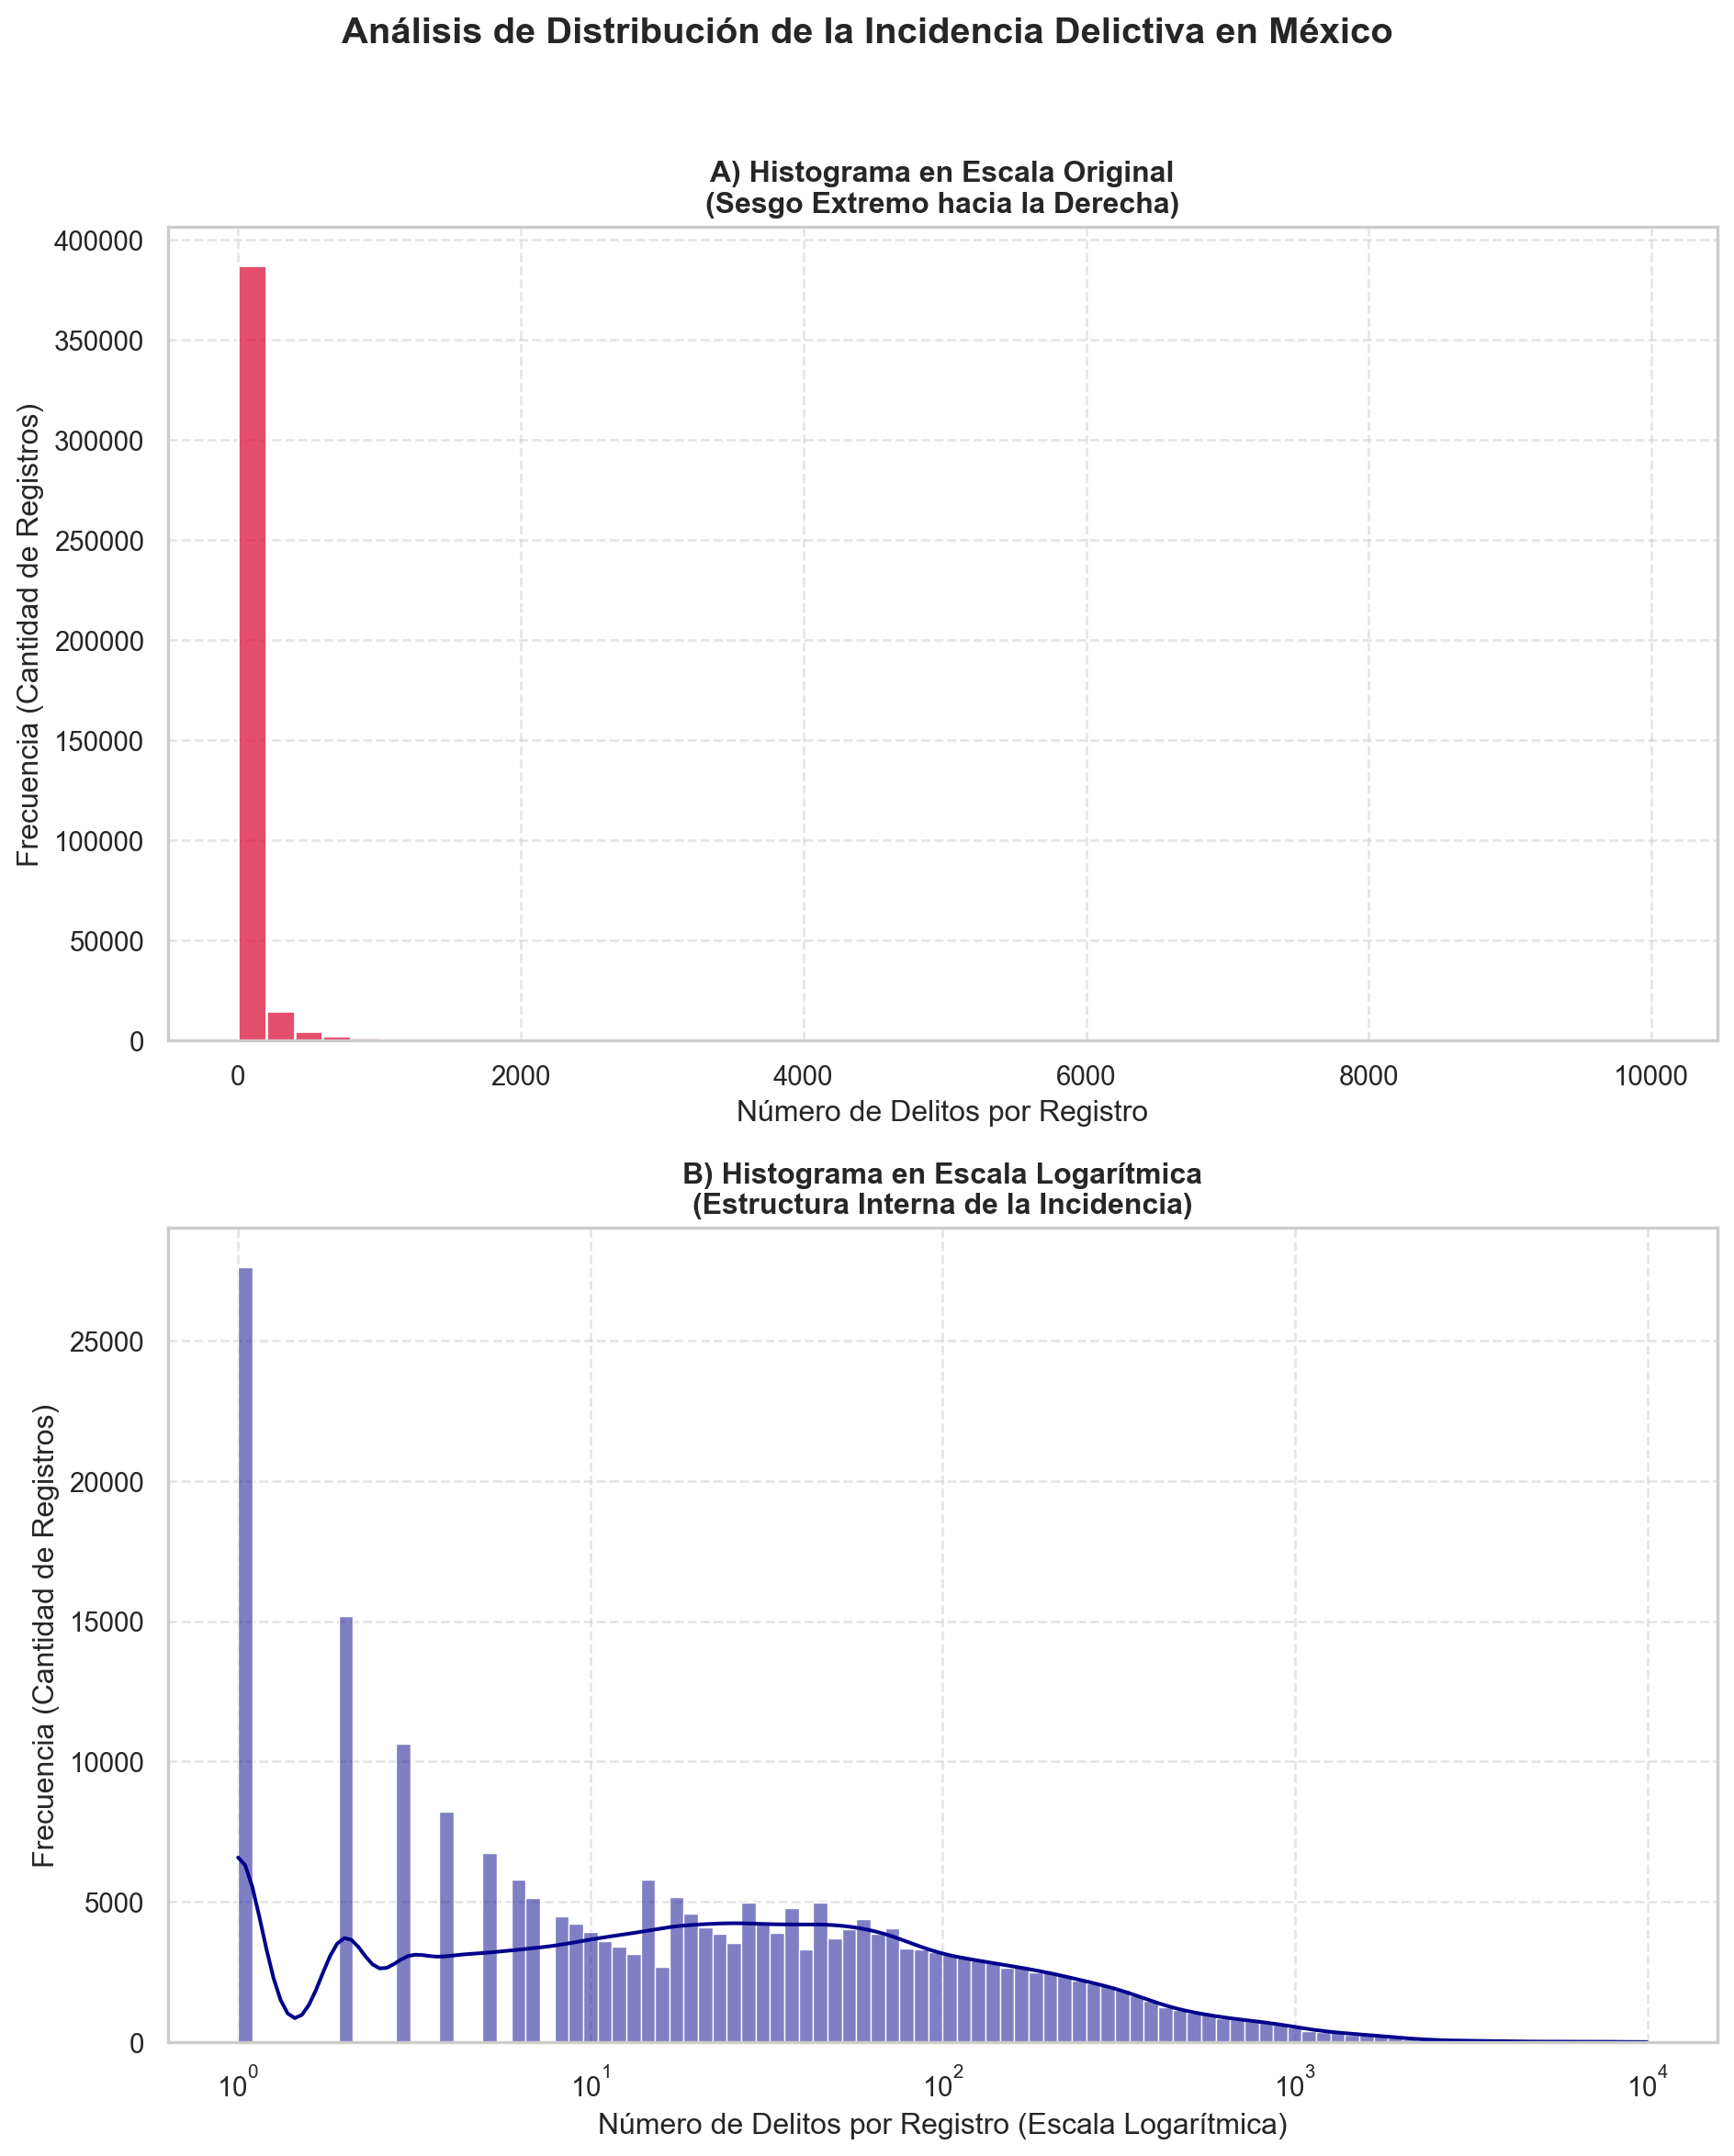
\includegraphics[width=0.75\textwidth]{imagenes/delective-incidence-histograms-output-1.png}
  \caption{Histogramas de Incidencia Delictiva por Estado (marcador de posición)}
  \label{fig:incidence-histograms}
\end{figure}

El primer gráfico muestra una distribución con un sesgo hacia la derecha extremadamente severa. La inmensa mayoría de los registros
del dataset se concentran de forma masiva en valores muy cercanos a cero (recordemos que la mediana del dataset es de 2 delitos por registro).
Esto se debe a que existen muchas categorías de delitos poco comunes o entidades con menor población que reportan frecuentemente cero u
muy pocas incidencias mensuales de estos delitos no tan comúnes. Visualmente, esto genera una gran "pared" en el extremo izquierdo
y una cola invisible infinitamente larga hacia la derecha que se extiende hasta el valor máximo de 9,968.

Con el segundo gráfico queremos reevelar la distribución real que queda oculta bajo el sesgo. Para esto se aplicó una escala logarítmica
sobre el eje de las abscisas (filtrando los registros con elitos). Esto nos da distribución con dos picos:

\begin{itemize}
  \item El primero muestra cuando se registran de 1 a 3 delitos en promedio. Esto representa la gran masa de reportes delictivos de baja
ocurrencia o zonas con baja densidad demográfica.
  \item El segundo muestra cuando se registran de 30 a 100 delitos en promedio. Esto representa la acumulación de delitos altamente recurrentes
(como variantes de robos) en zonas urbanas o de alta incidencia.
\end{itemize}

\subsection{Estadísticas Descriptivas Categóricas}

\begin{lstlisting}[language=Python, caption={Código para obtener estadísticas descriptivas categóricas}, label={lst:stats-descriptivas-categoricas}]
	stats.categorical_stats()
\end{lstlisting}

\begin{table}[ht]
  \centering
  \caption{Estadísticas Descriptivas Categóricas}
  \scriptsize
  \resizebox{\textwidth}{!}{%
    \begin{tabular}{r r r l p{3.5cm} p{3cm} p{3cm} p{2.5cm} l l r l}
      \hline
      \textbf{idx} & \textbf{columna} & \textbf{valores únicos} & \textbf{moda} & \textbf{frecuencia modal} \\
      0 & fecha & 132 & 2015-04-01 & 3136 \\
      1 & entidad & 32 & Aguascalientes & 12936 \\
      2 & bien\_juridico\_afectado & 7 & El patrimonio & 177408 \\
      3 & tipo\_delito & 40 & Robo & 152064 \\
      4 & subtipo\_delito & 55 & Robo de maquinaria & 25344 \\
      5 & modalidad & 59 & Con violencia & 50688 \\
      \hline
    \end{tabular}%
  }
  \label{tab:categorical-stats}
\end{table}

En cuanto a las variables categóricas del conjunto de datos podemos notar hechos bastante interesantes a pesar de la inmensidad del dataset:

\begin{itemize}
  \item El dataset es de 11 años, sin embargo, solo hay 132 fechas únicas, con la fecha inicial siendo el 01 de enero de 2015
  \item La moda del dataset tiene algunos resultados curiosos. Este conjunto de datos es simetrico para cada estado, ya que existen 12936
líneas para c/u. Entonces, al querer cálcular la moda se toma el valor inicial de manera alfabética y resulta ser Aguascalientes.
Sin embargo, esto no significa que sea la entidad con mayor apariciones del dataset.
  \item Lo anterior pasa de igual manera con la fecha, ya que toma la primera fecha del dataset para calcular este valor.
  \item El dataset reporta 40 tipos de delitos únicos reportados, con Robo siendo la categoría principal.
\end{itemize}

Veamos ahora un análisis más detallado de las variables categóricas.

\subsubsection{Delitos más Comunes}

\begin{lstlisting}[language=Python, caption={Código para generar gráfico de los delitos más comunes}, label={lst:delitos-mas-comunes}]
crime_counts = dataframe["tipo_delito"].value_counts().head(10)

fig, ax = plt.subplots(figsize=(10, 4))
crime_counts.plot(kind="barh", ax=ax, color="steelblue")
ax.set_title("Top 10 Tipos de Delito", fontsize=13, fontweight="bold")
ax.set_xlabel("Número de Registros")
ax.invert_yaxis()

# Añade valores en las barras
for i, v in enumerate(crime_counts.values):
    ax.text(v + 1000, i, f"{v:,}", va="center", fontsize=10)

plt.tight_layout()
plt.show()
\end{lstlisting}

\begin{figure}[H]
  \centering
  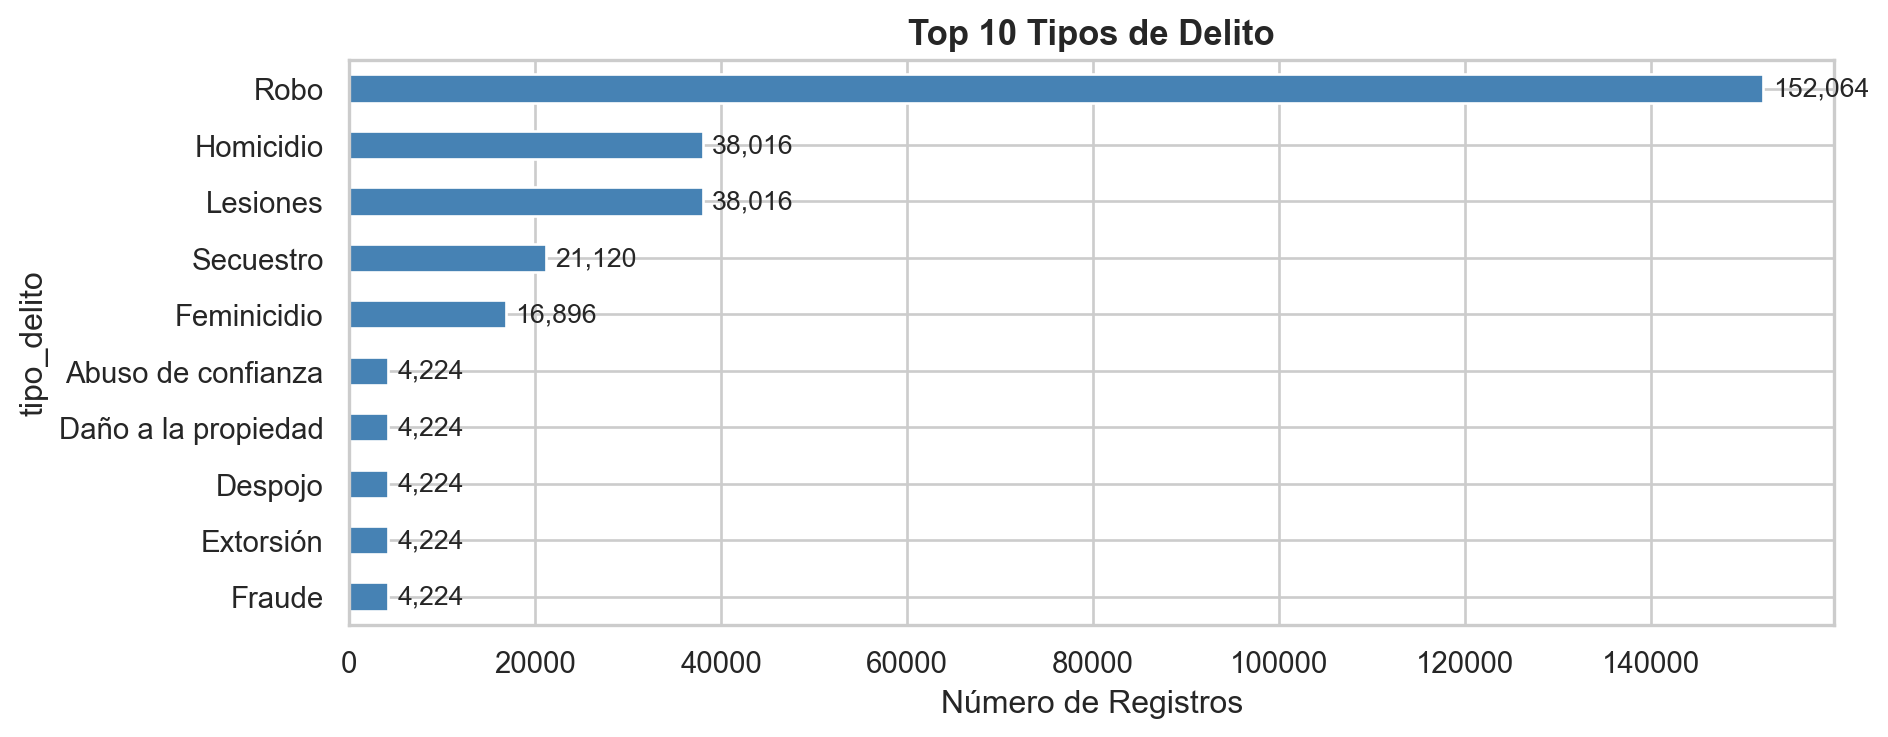
\includegraphics[width=0.85\textwidth]{imagenes/most-common-crimes-output-1.png}
  \caption{Top 10 Tipos de Delito}
  \label{fig:top-crimes}
\end{figure}

Como se mencionaba en la tabla anterior, robo es el delito más reportado, seguido de homicidio y lesiones. Algo a recordar
es que aunque los feminicidios son también homicidios éstos están en una categoriá separada debido al motivo por el que ocurren.
Vemos también que hay una extraña coincidencia de valores entre Abuso de Confianza, Daño a la Propiedad, Despojo, Extorsión y Fraude,
lo que sugiere un sesgo al momento de reportar estos delitos por parte de la autoridad (por ejemplo, cifras redondeadas, reportes nulos, etc.)

\subsubsection{Incidencia Delictiva por Estado}

\begin{lstlisting}[language=Python, caption={Código para generar gráfico de incidencia delictiva por estado}, label={lst:incidencia-delictiva-por-estado}]
from matplotlib.ticker import StrMethodFormatter

entidad_counts = (
    dataframe.groupby("entidad")["incidencia_delictiva"]
    .sum()
    .sort_values(ascending=False)
    .head(10)
)

fig, ax = plt.subplots(figsize=(10, 6))
bars = ax.bar(entidad_counts.index, entidad_counts.values, color="coral")
# Formato del eje Y con separadores de miles y sin decimales
ax.yaxis.set_major_formatter(StrMethodFormatter("{x:,.0f}"))
# Agregamos los valores reales arriba de cada barra con separadores de miles
ax.bar_label(bars, fmt="{:,.0f}", padding=3, fontsize=10, fontweight="bold")

ax.set_title(
    "Incidencia Delictiva Total por Entidad (Top 10) - 2015 a 2025",
    fontsize=15,
    fontweight="bold",
    pad=15,
)
ax.set_ylabel("Total de Delitos", fontsize=12)
ax.set_xlabel("Entidad Federativa", fontsize=12)
ax.tick_params(axis="x", rotation=40)

plt.tight_layout()
plt.show()
\end{lstlisting}

\begin{figure}[H]
  \centering
  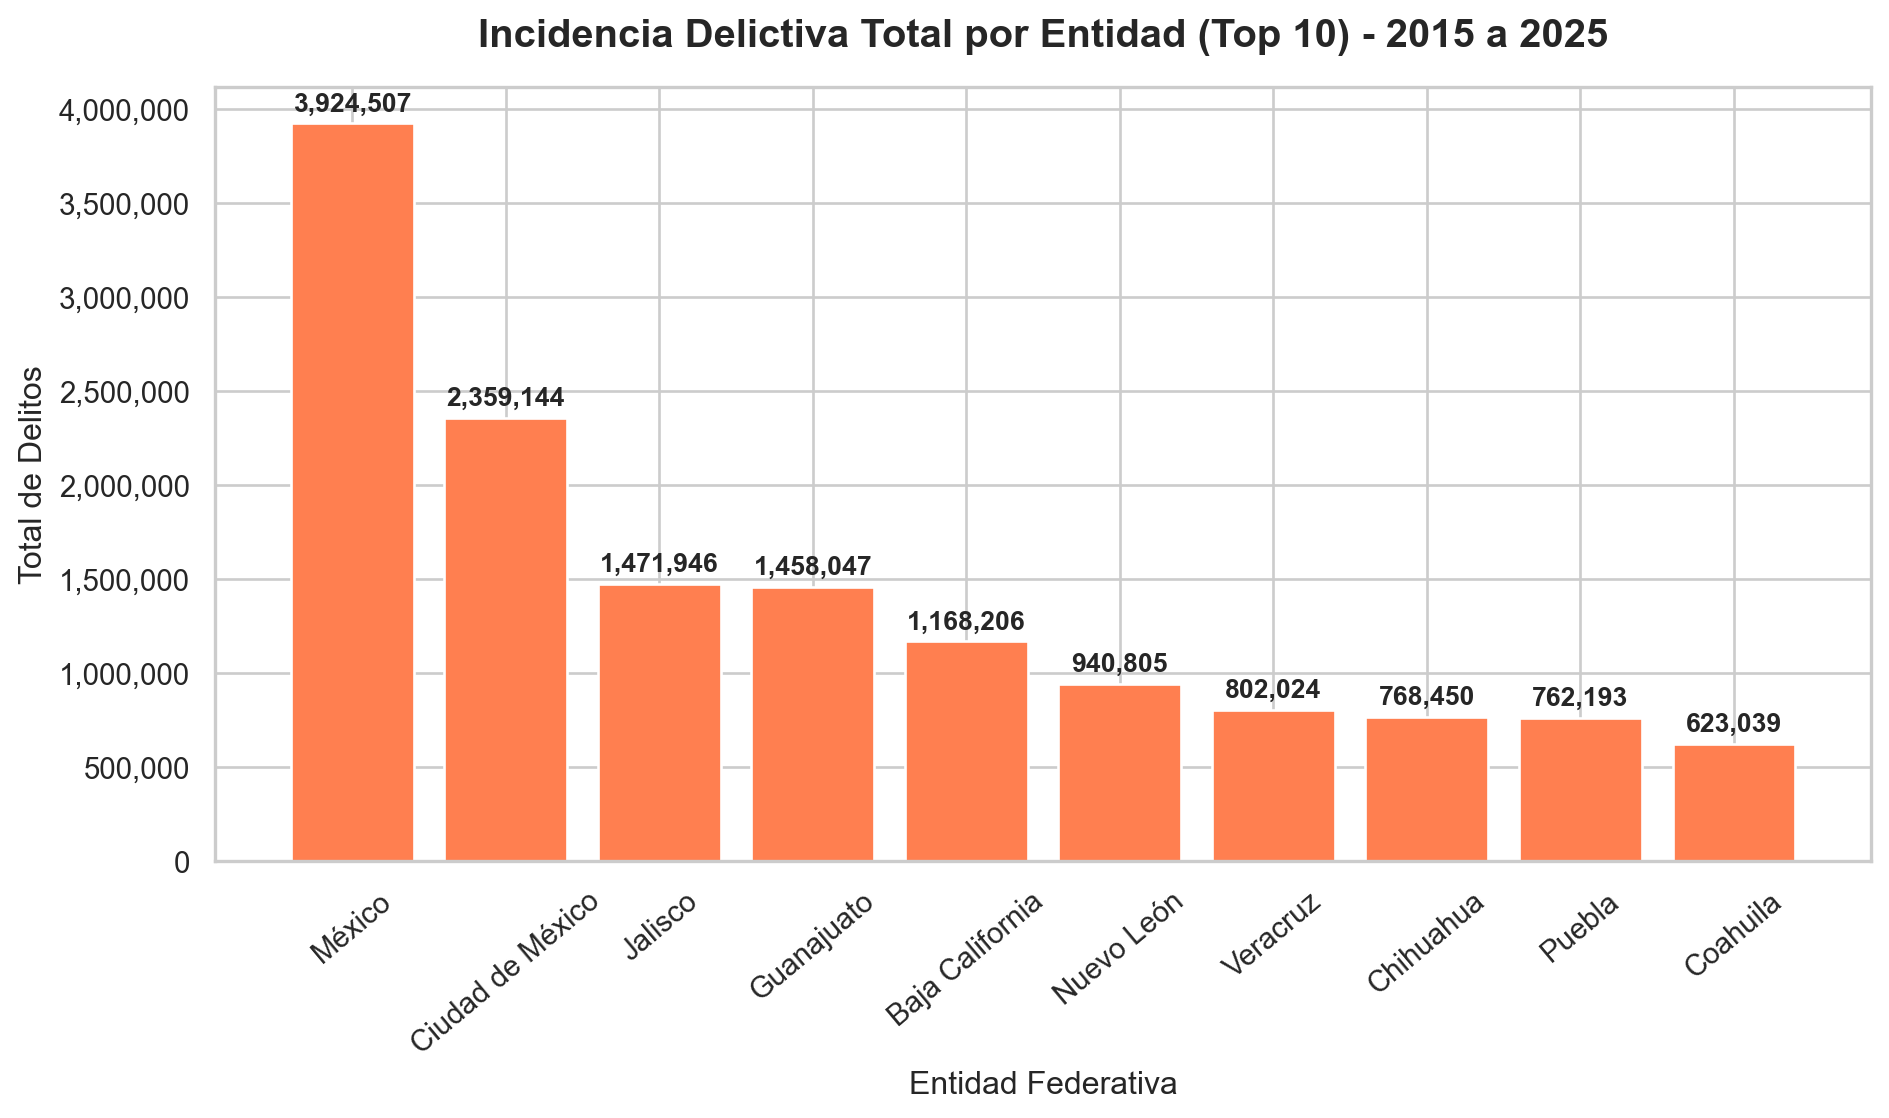
\includegraphics[width=0.8\textwidth]{imagenes/crime-by-state-output-1.png}
  \caption{Incidencia Delictiva Total por Entidad}
  \label{fig:crime-by-state}
\end{figure}

Nuestra sospecha anterior que la EdoMex y la CDMX son los estados con más reportes es correcta. Vemos que le siguen Jalisco,
Guanajuato y Baja California y que, a pesar de la moda, Aguascalientes no figura dentro de los estados con más delitos reportados.

\begin{lstlisting}[language=Python, caption={Código para generar mapa de calor de incidencia por entidad y tipo de delito}, label={lst:heatmap-incidencia-por-entidad-y-delito}]
top_crimes = dataframe["tipo_delito"].value_counts().head(10).index
top_entities = dataframe["entidad"].value_counts().head(10).index

filtered_df = dataframe[dataframe["tipo_delito"].isin(top_crimes) & dataframe["entidad"].isin(top_entities)]

pivot = filtered_df.pivot_table(
    values="incidencia_delictiva", index="entidad", columns="tipo_delito", aggfunc="sum"
)

fig, ax = plt.subplots(figsize=(10, 10))
sns.heatmap(
    pivot,
    cmap="RdYlGn_r",
    annot=True,
    fmt=",.0f",  # Agregamos la coma para que los números dentro del mapa tengan comas (ej. 1,234,567)
    cbar_kws={"label": "Incidencia"},
    ax=ax,
)

cbar = ax.collections[0].colorbar
# aplicamos formato con comas de miles y sin decimales
cbar.ax.yaxis.set_major_formatter(StrMethodFormatter('{x:,.0f}'))

ax.set_title(
    "Incidencia por Entidad y Tipo de Delito",
    fontsize=12,
    fontweight="bold",
    pad=15
)

plt.tight_layout()
plt.show()
\end{lstlisting}

\begin{figure}[H]
  \centering
  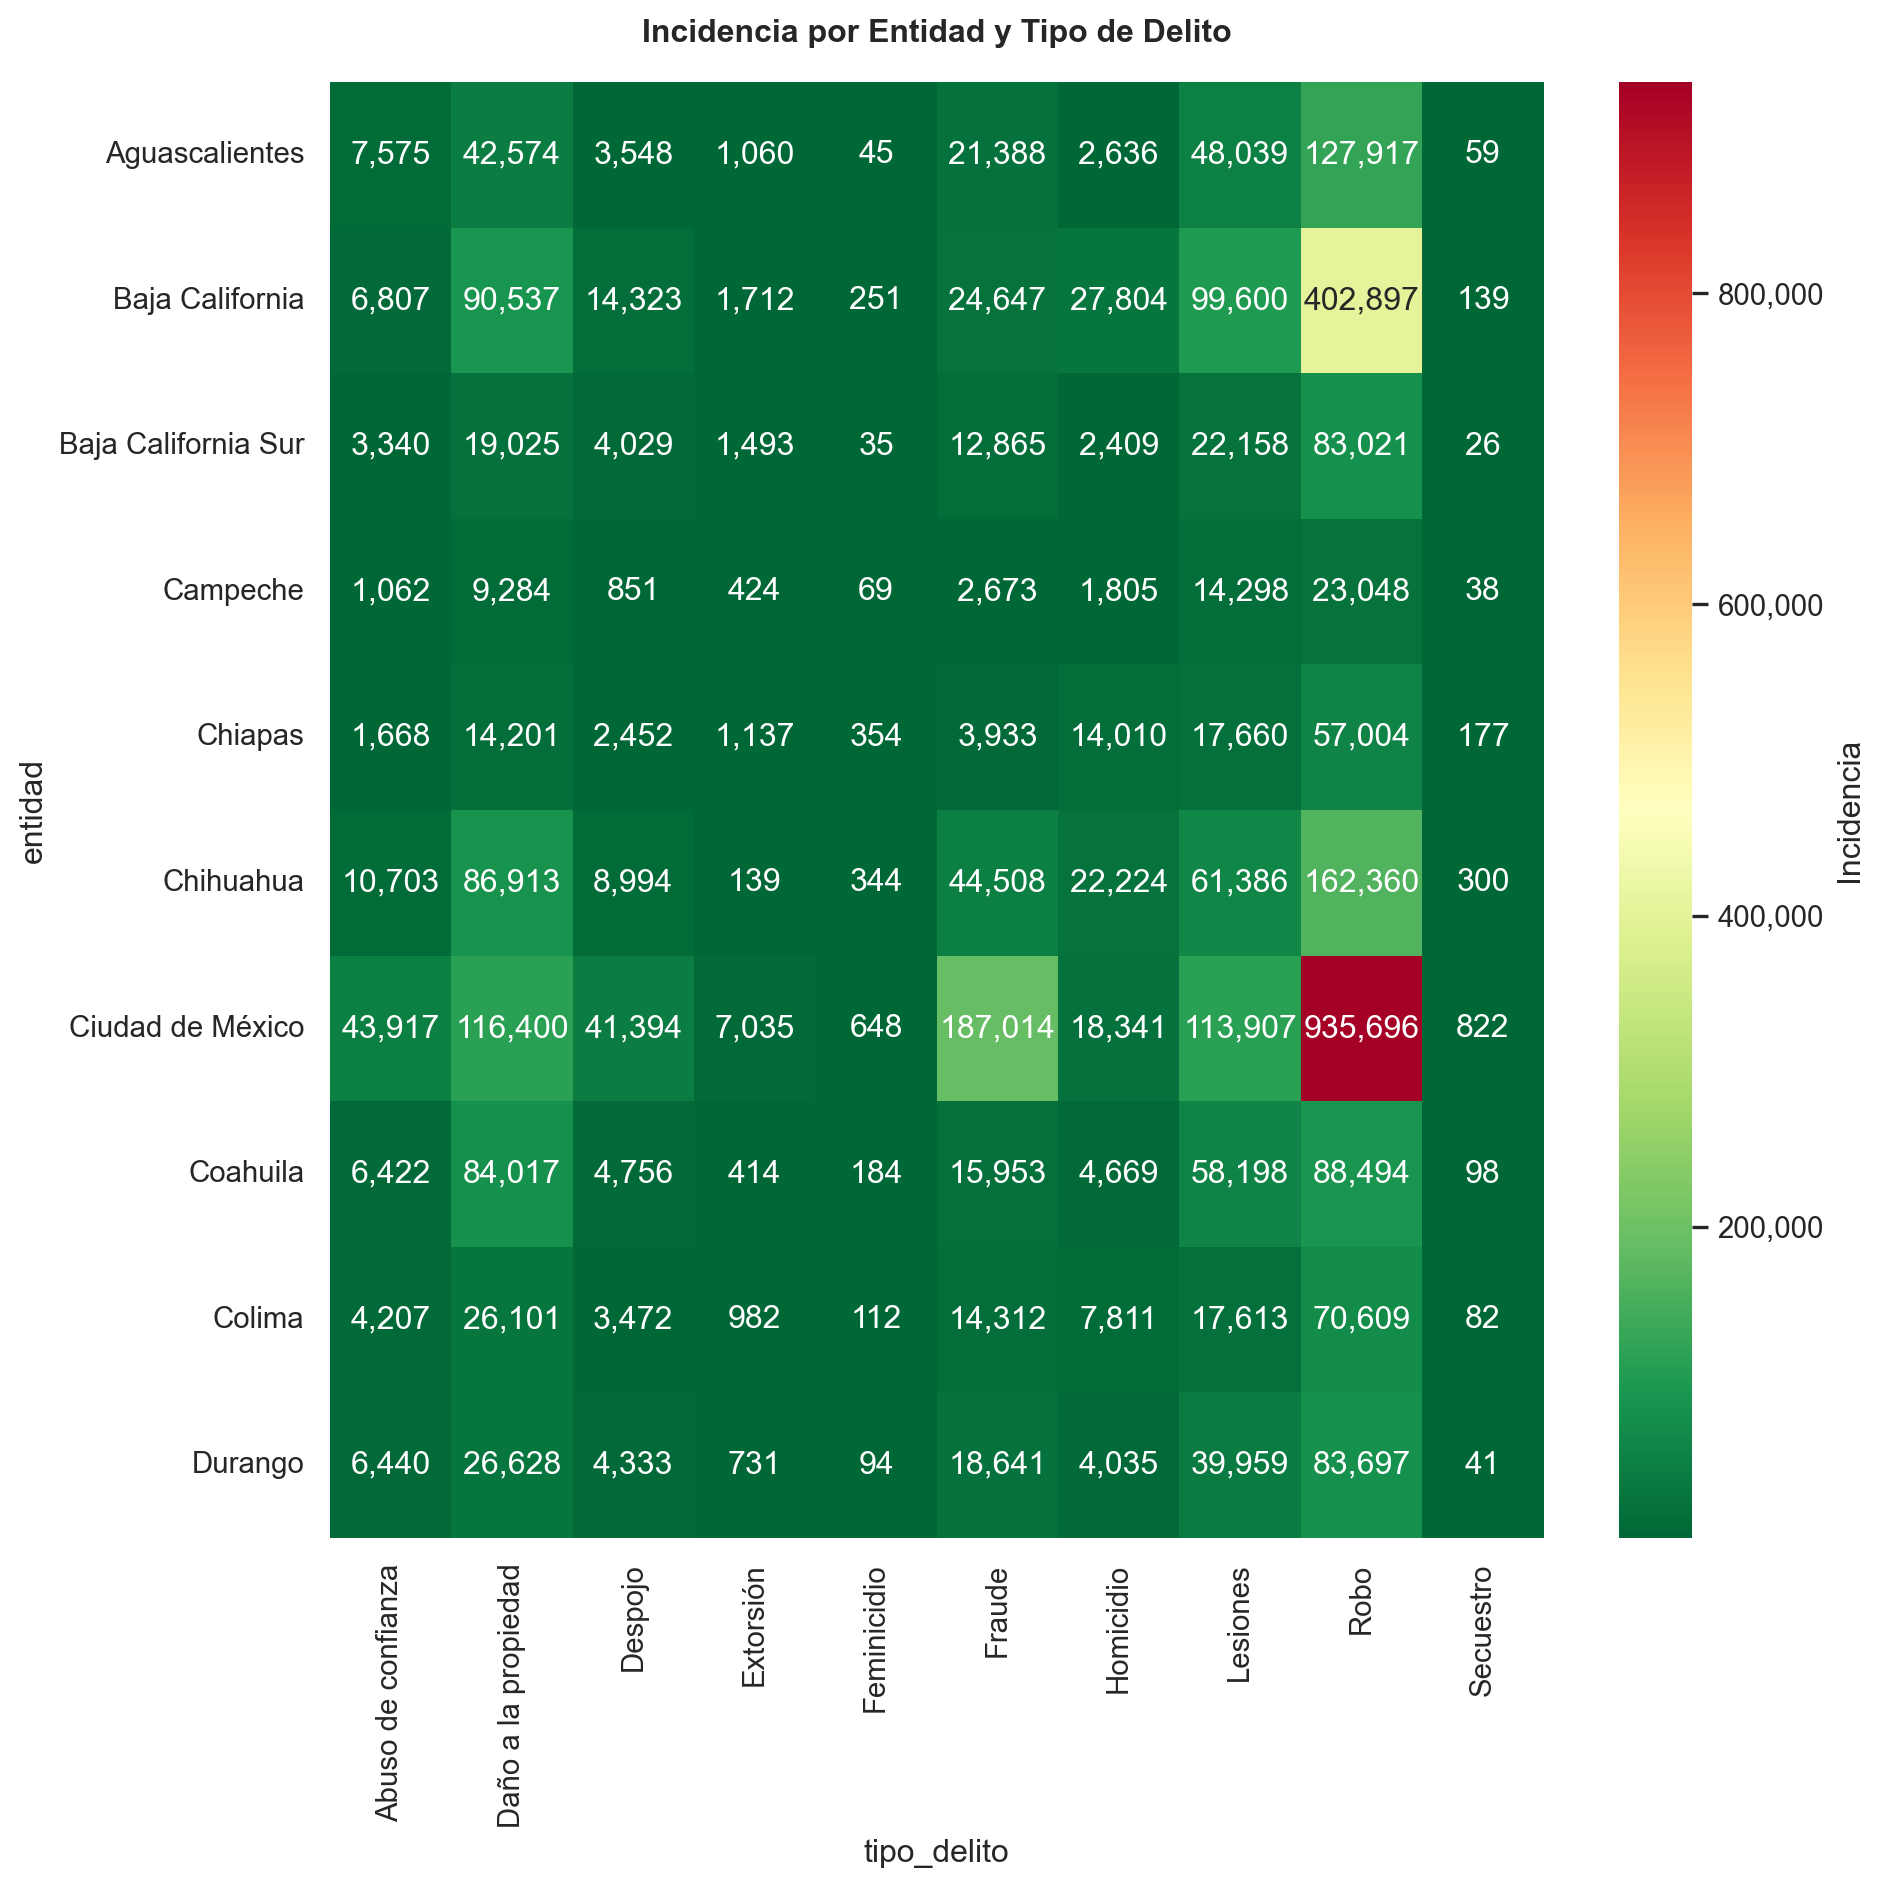
\includegraphics[width=0.8\textwidth]{imagenes/crime-heatmap-output-1.png}
  \caption{Mapa de calor de incidencia por entidad y tipo de delito}
  \label{fig:crime-heatmap}
\end{figure}

\subsubsection{Bienes Jurídicos más Afectados}

\begin{lstlisting}[language=Python, caption={Código para generar gráfico de bienes jurídicos más afectados}, label={lst:bienes-juridicos-mas-afectados}]
bien_juridico = dataframe["bien_juridico_afectado"].value_counts()

fig, ax = plt.subplots(figsize=(8, 8))
wedges, texts, autotexts = ax.pie(
    bien_juridico.values, labels=bien_juridico.index, autopct="%1.1f%%", startangle=90
)
ax.set_title(
    "Distribución de Delitos por Bien Jurídico Afectado", fontsize=11, fontweight="bold"
)
for autotext in autotexts:
    autotext.set_color("white")

plt.show()
\end{lstlisting}

\begin{figure}[H]
	\centering
	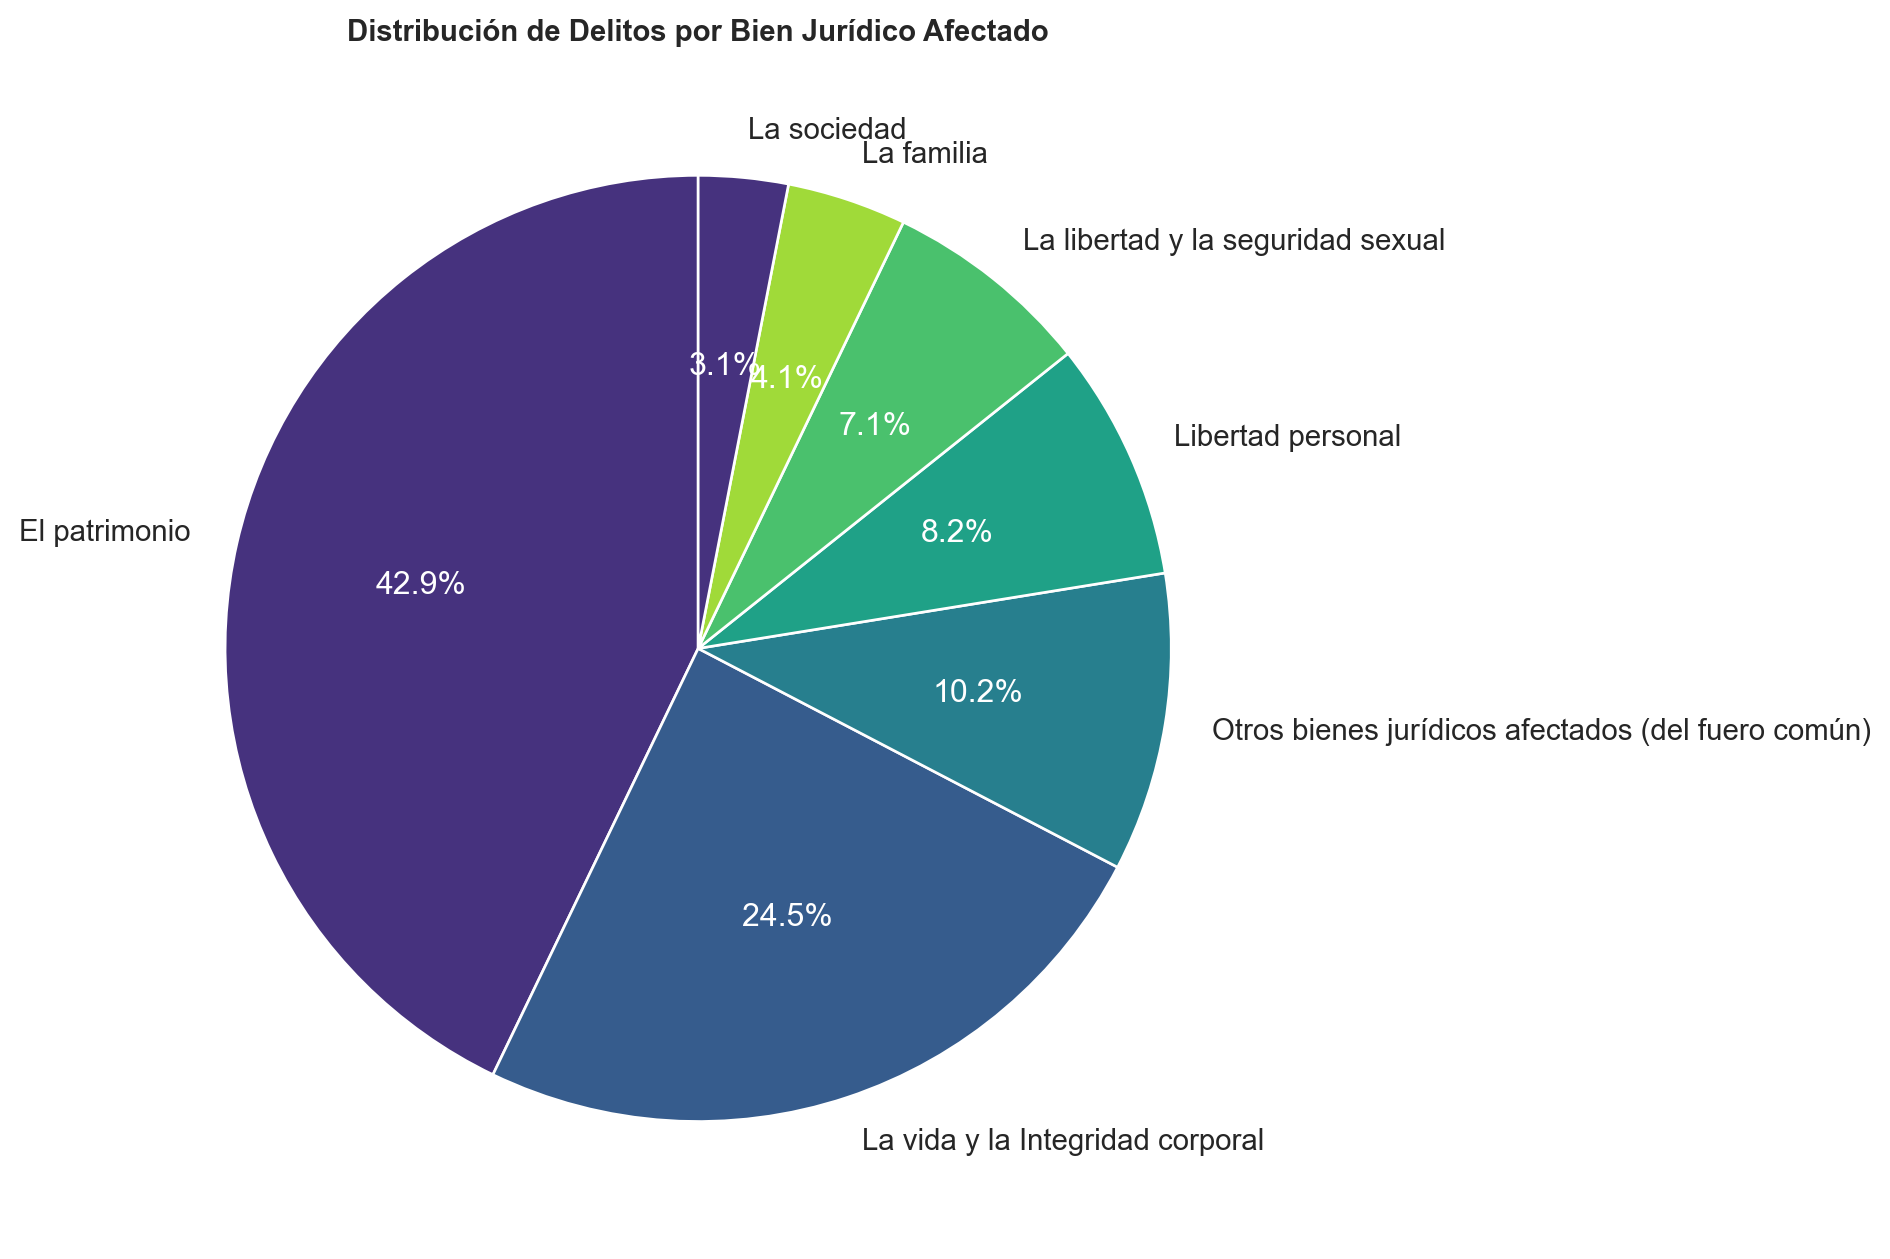
\includegraphics[width=0.75\textwidth]{imagenes/affected-legal-assets-output-1.png}
	\caption{Bienes Jurídicos más Afectados por Delitos en México (2015-2025)}
	\label{fig:affected-legal-assets}
\end{figure}

Para entender esta gráfica debemos entender que la ley define como ‘bienes jurídicos’ a aquellos objetos o relaciones, tangibles o intangibles, que
cuentan con la protección de la ley, como un inmueble, la vida, dinero, etc. En particular, debemos entender que 'El patrimonio' hace referencia al
conjunto de bienes, derechos y obligaciones de una persona, susceptibles de valoración económica. Lo anterior, en otros términos, se refiere a
pertenencias que hemos comprado, dinero que tenga un individuo, etc, pero que tengan relevancia ecónomica.

Ahora pues, tomando en cuenta de que el delito más reportado es el robo, que el patrimonio sea el bien más afectado tiene mucho sentido. Luego, al
ser el homicidio, lesiones, secuestro y feminicidio los delitos que siguen en frecuencia, hace nuevamente sentido que la vida e integridad corportal
sean el segundo bien más afectado.

\subsubsection{Modalidad de los Delitos}

\begin{lstlisting}[language=Python, caption={Código para generar gráfico de modalidades de los delitos}, label={lst:modalidades-delitos}]
modalidad = dataframe["modalidad"].value_counts().head(15)

fig, ax = plt.subplots(figsize=(10, 10))
modalidad.plot(kind="barh", ax=ax, color=["#d62728", "#2ca02c"])

ax.set_title("Distribución de Delitos por Modalidad (Top 10, 2015-2025)", fontsize=10, fontweight="bold")
ax.set_xlabel("Número de Registros")

for i, v in enumerate(modalidad.values):
    ax.text(v + 500, i, f"{v:,}", va="center")

plt.tight_layout()
plt.show()
\end{lstlisting}

\begin{figure}[H]
    \centering
    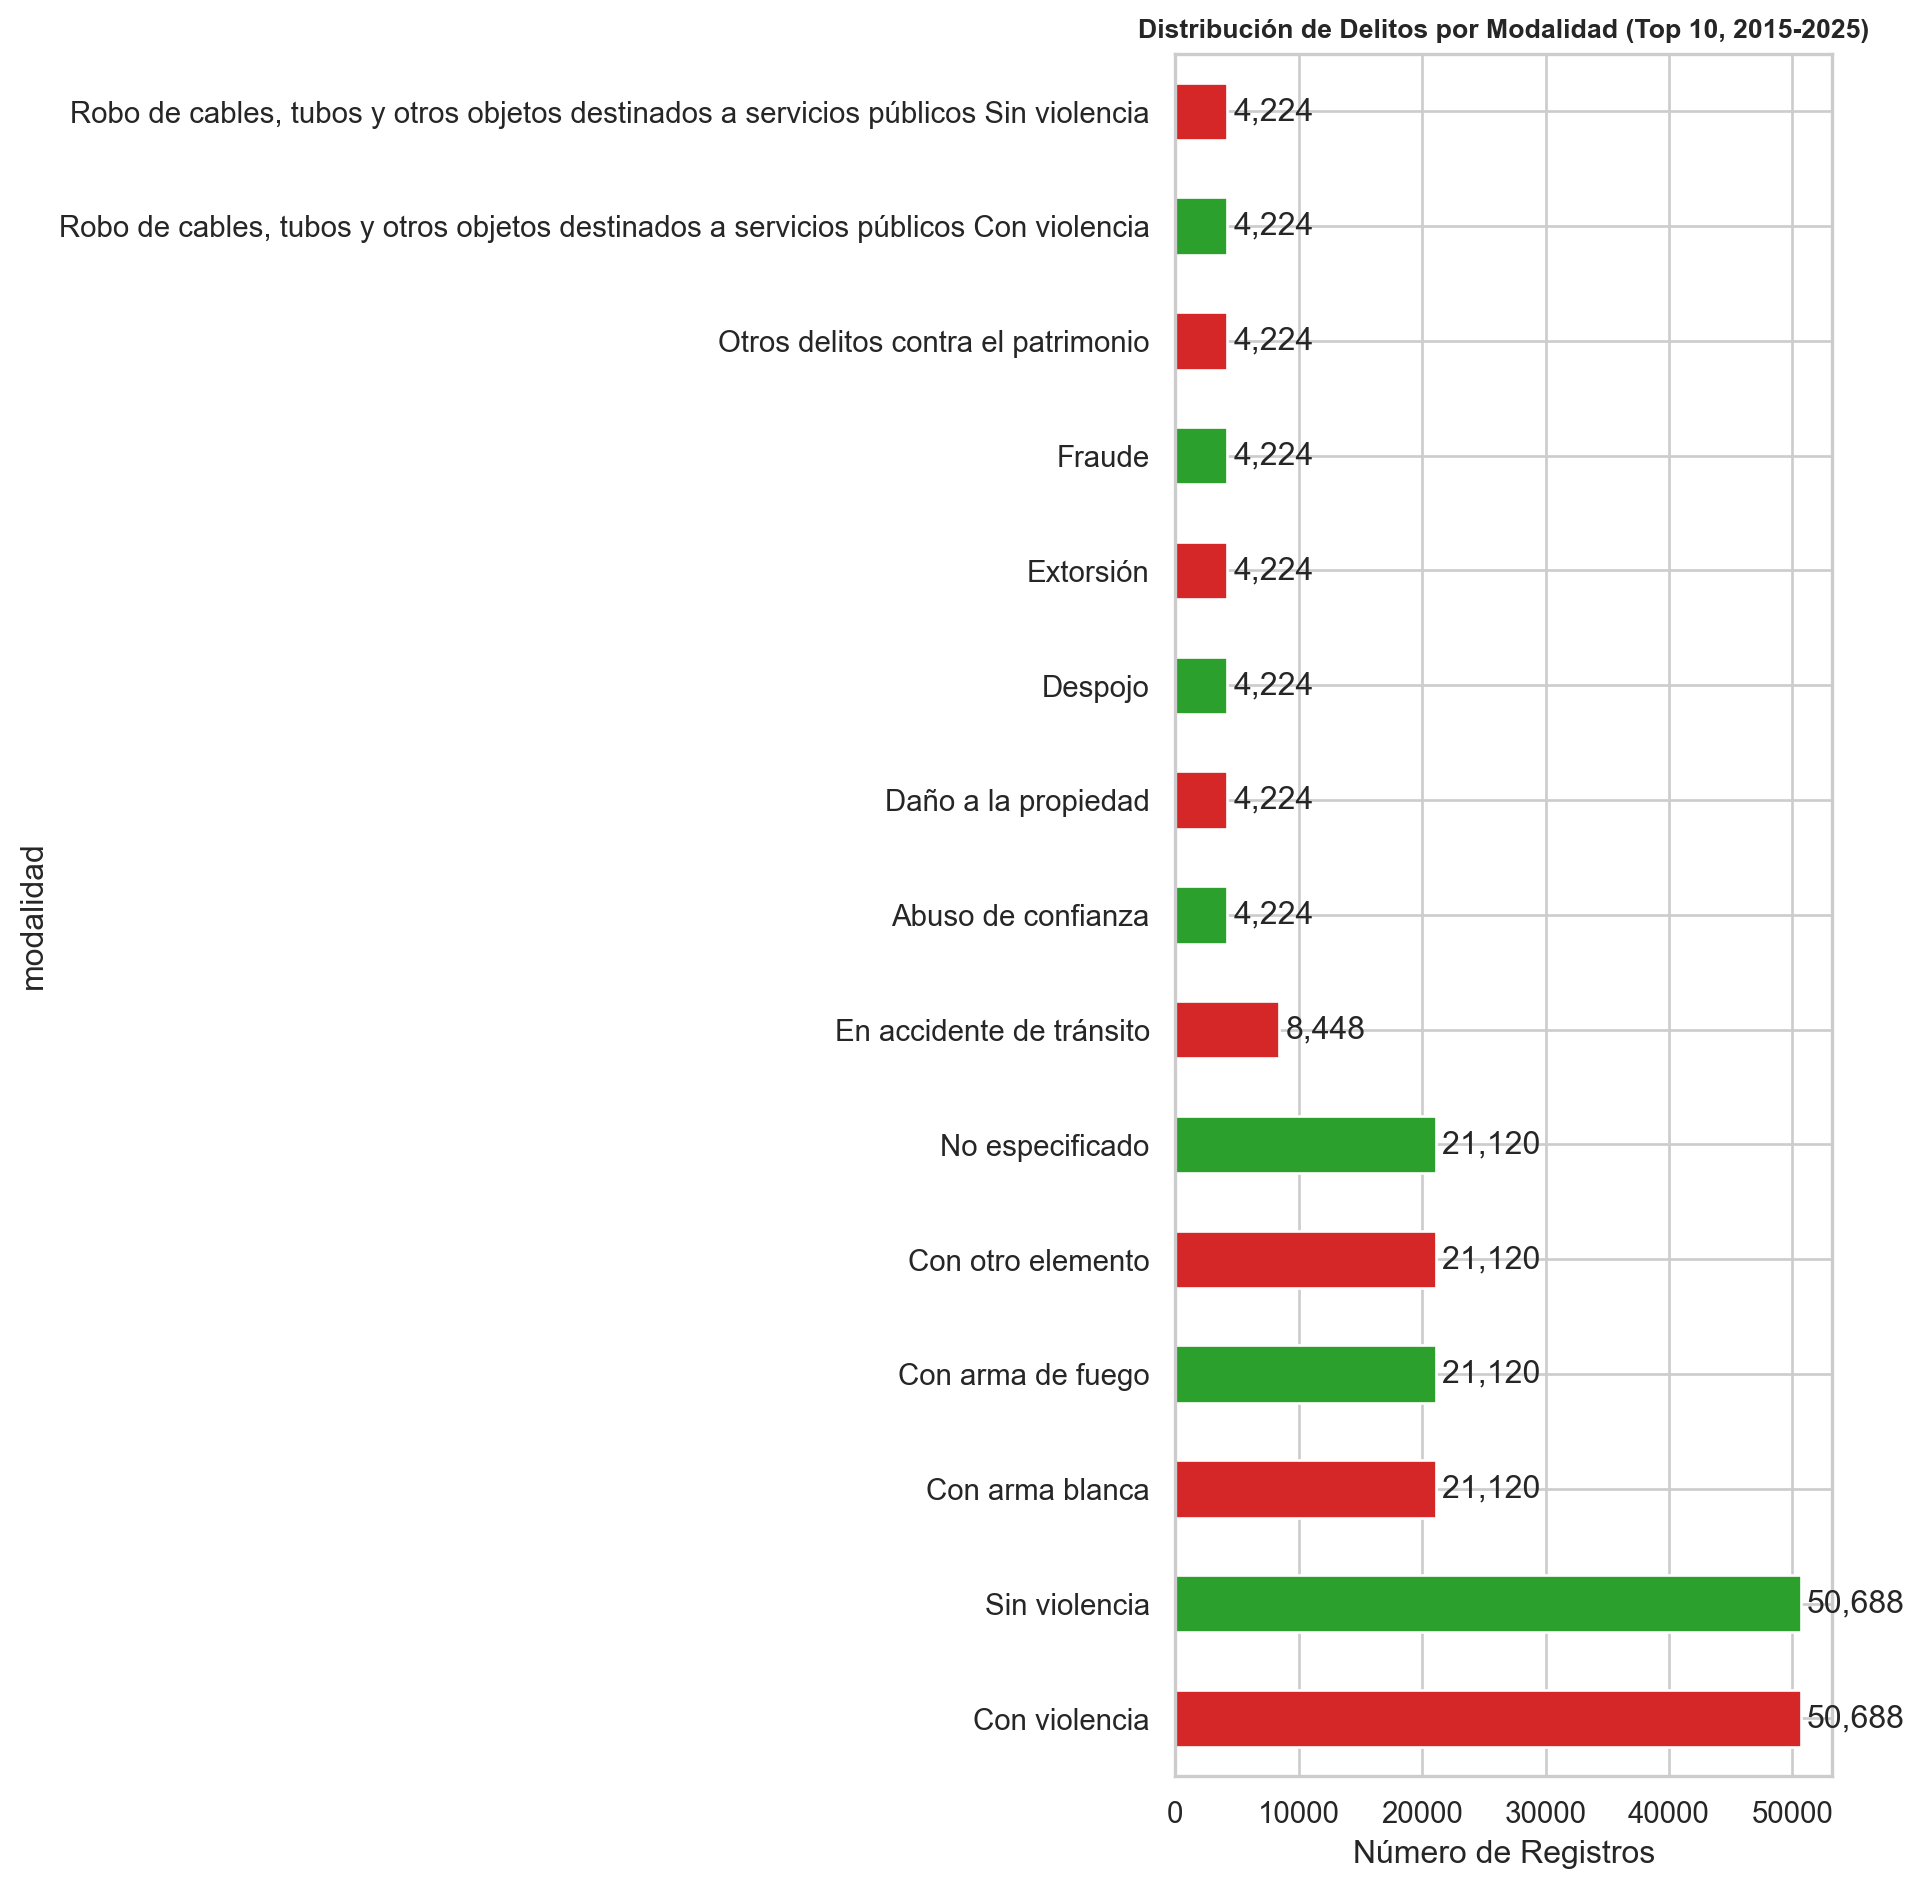
\includegraphics[width=0.7\textwidth]{imagenes/crime-modality-output-1.png}
    \caption{Modalidad de los Delitos en México (2015-2025)}
    \label{fig:crime-modalities}
\end{figure}

Nuevamente, vemos también que hay una extranña coincidencia de valores después de la modalidad ‘En Accidente
de Tráfico’, lo que sugiere y mantiene la idea de que existe un gran sesgo al momento de reportar correctamente
todos los delitos.

También notamos que no existe una única forma de reportar los delitos con violencia, por lo que un registro
puede pertenecer a un delito con ésta modalidad y ser asignado a otra categoria (sobre todo en lo referente
a los subtipos de robo).

\subsubsection{Delincuencia por Año}

\begin{lstlisting}[language=Python, caption={Código para generar gráfico de delincuencia por año}, label={lst:delincuencia-por-año}]
dataframe["fecha"] = pd.to_datetime(dataframe["fecha"])  # add this line before groupby
temporal = dataframe.groupby("fecha")["incidencia_delictiva"].sum().sort_index()

fig, ax = plt.subplots(figsize=(10, 6))
ax.plot(temporal.index, temporal.values, linewidth=2, color="darkred")
ax.fill_between(temporal.index, temporal.values, alpha=0.2, color="red")

ax.set_title(
    "Evolución Temporal de la Incidencia Delictiva (2015-2025)",
    fontsize=13,
    fontweight="bold",
)
ax.set_xlabel("Fecha")
ax.set_ylabel("Incidencia Delictiva Total")
ax.grid(True, alpha=0.2)
ax.xaxis.set_major_locator(mdates.YearLocator())
ax.xaxis.set_major_formatter(mdates.DateFormatter("%Y"))
ax.xaxis.set_minor_locator(mdates.MonthLocator())
ax.grid(True, which="major", alpha=0.3)
ax.grid(True, which="minor", alpha=0.1)
plt.tight_layout()
plt.show()
```
\end{lstlisting}

\begin{figure}[H]
    \centering
    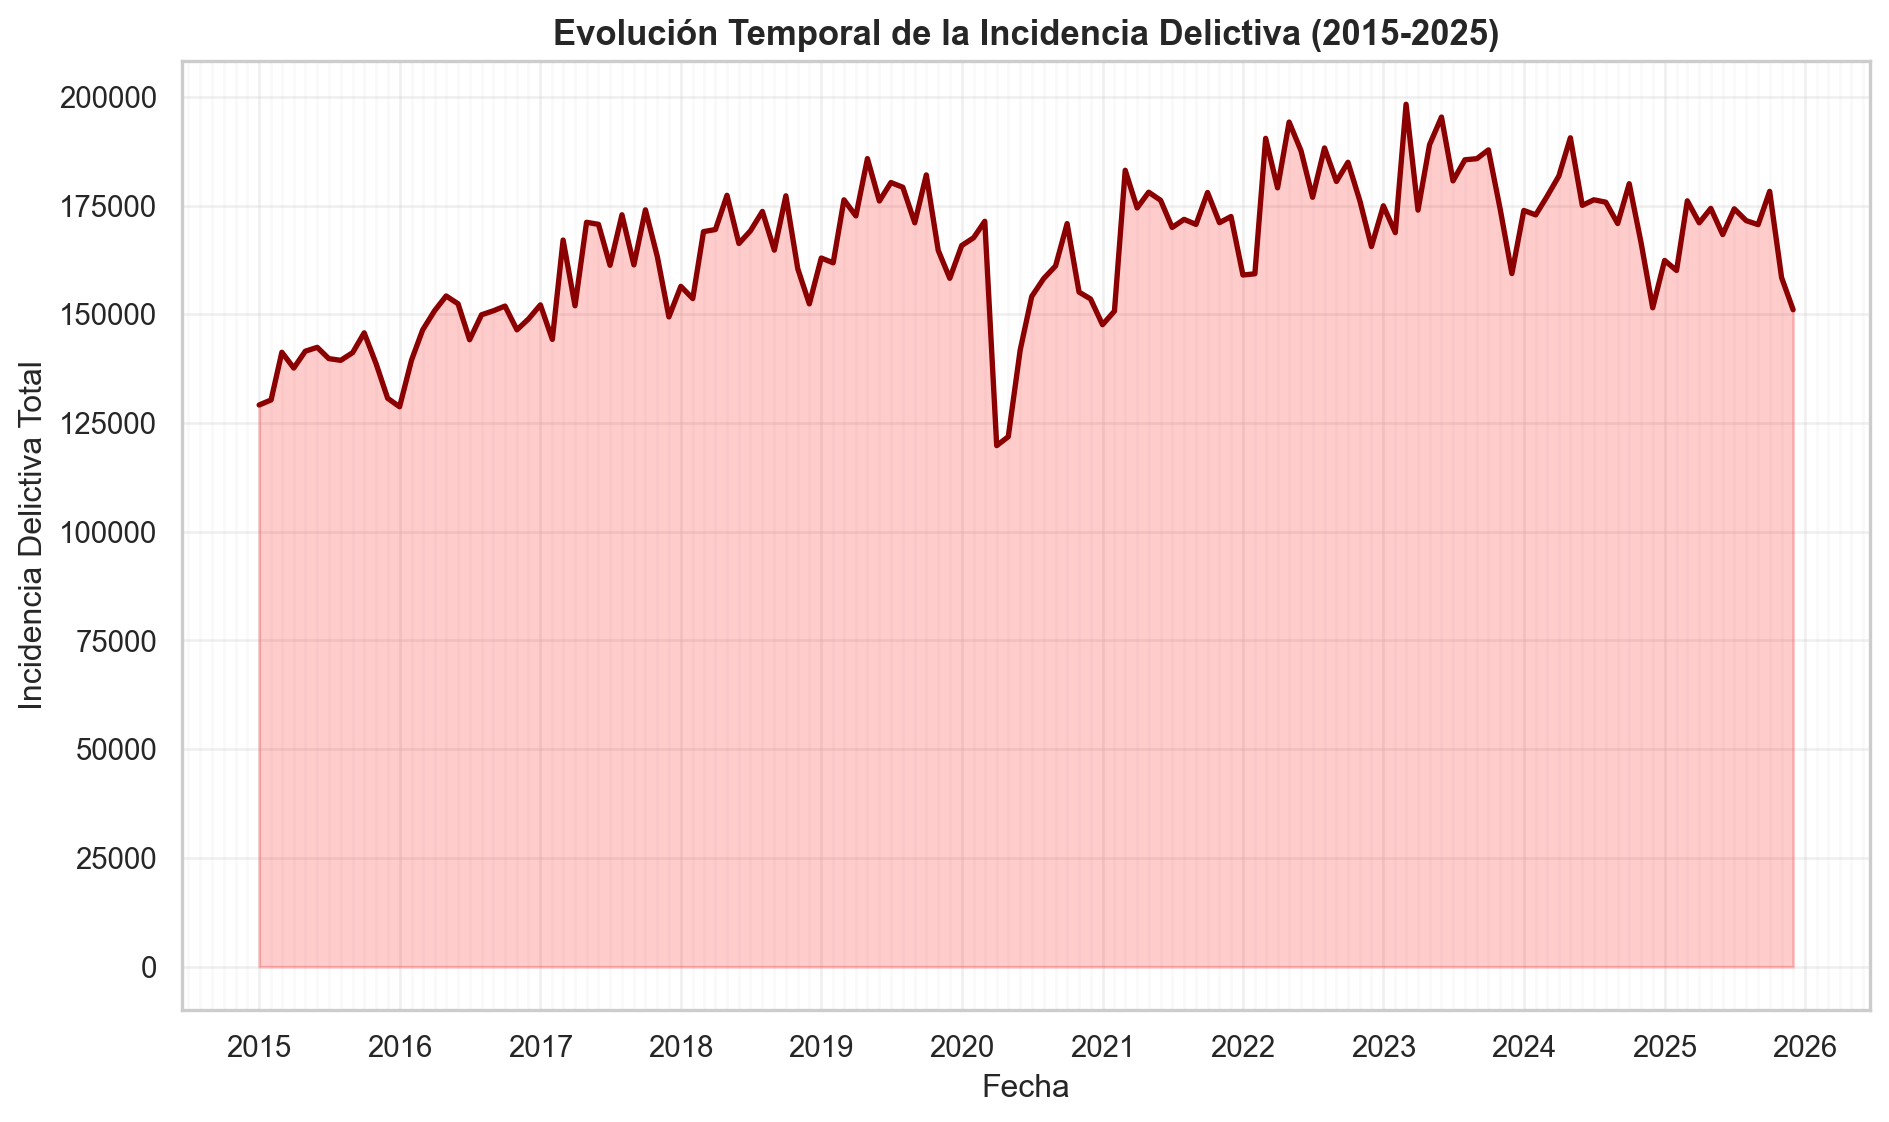
\includegraphics[width=0.8\textwidth]{imagenes/crime-by-year-output-1.png}
    \caption{Evolución Temporal de la Incidencia Delictiva en México (2015-2025)}
    \label{fig:crime-over-time}
\end{figure}

Vemos que, desafortunadamente, no existe un decrecimiento notable en cuanto a la delicuencia en este periodo de tiempo. E incluso, desde 2022
hacia adelante es donde se alcanzan números más alto.

Veamos ahora como se ve ésta evolución dados los meses del año:

\begin{lstlisting}[language=Python, caption={Código para generar gráfico de delincuencia por mes}, label={lst:delincuencia-por-mes}]
dataframe["fecha"] = pd.to_datetime(dataframe["fecha"])
dataframe["año"] = dataframe["fecha"].dt.year
dataframe["mes"] = dataframe["fecha"].dt.month

pivot_data = dataframe.groupby(["año", "mes"])["incidencia_delictiva"].sum().unstack()

fig, ax = plt.subplots(figsize=(10, 10))
sns.heatmap(
    pivot_data,
    cmap="YlOrRd",
    annot=False,
    fmt="d",
    cbar_kws={"label": "Incidencia Delictiva"},
    ax=ax,
)

ax.set_title(
    "Patrón Mensual de Delincuencia por Año (2015-2025)", fontsize=13, fontweight="bold"
)
ax.set_xlabel("Mes")
ax.set_ylabel("Año")

plt.tight_layout()
plt.show()
\end{lstlisting}

\begin{figure}[H]
    \centering
    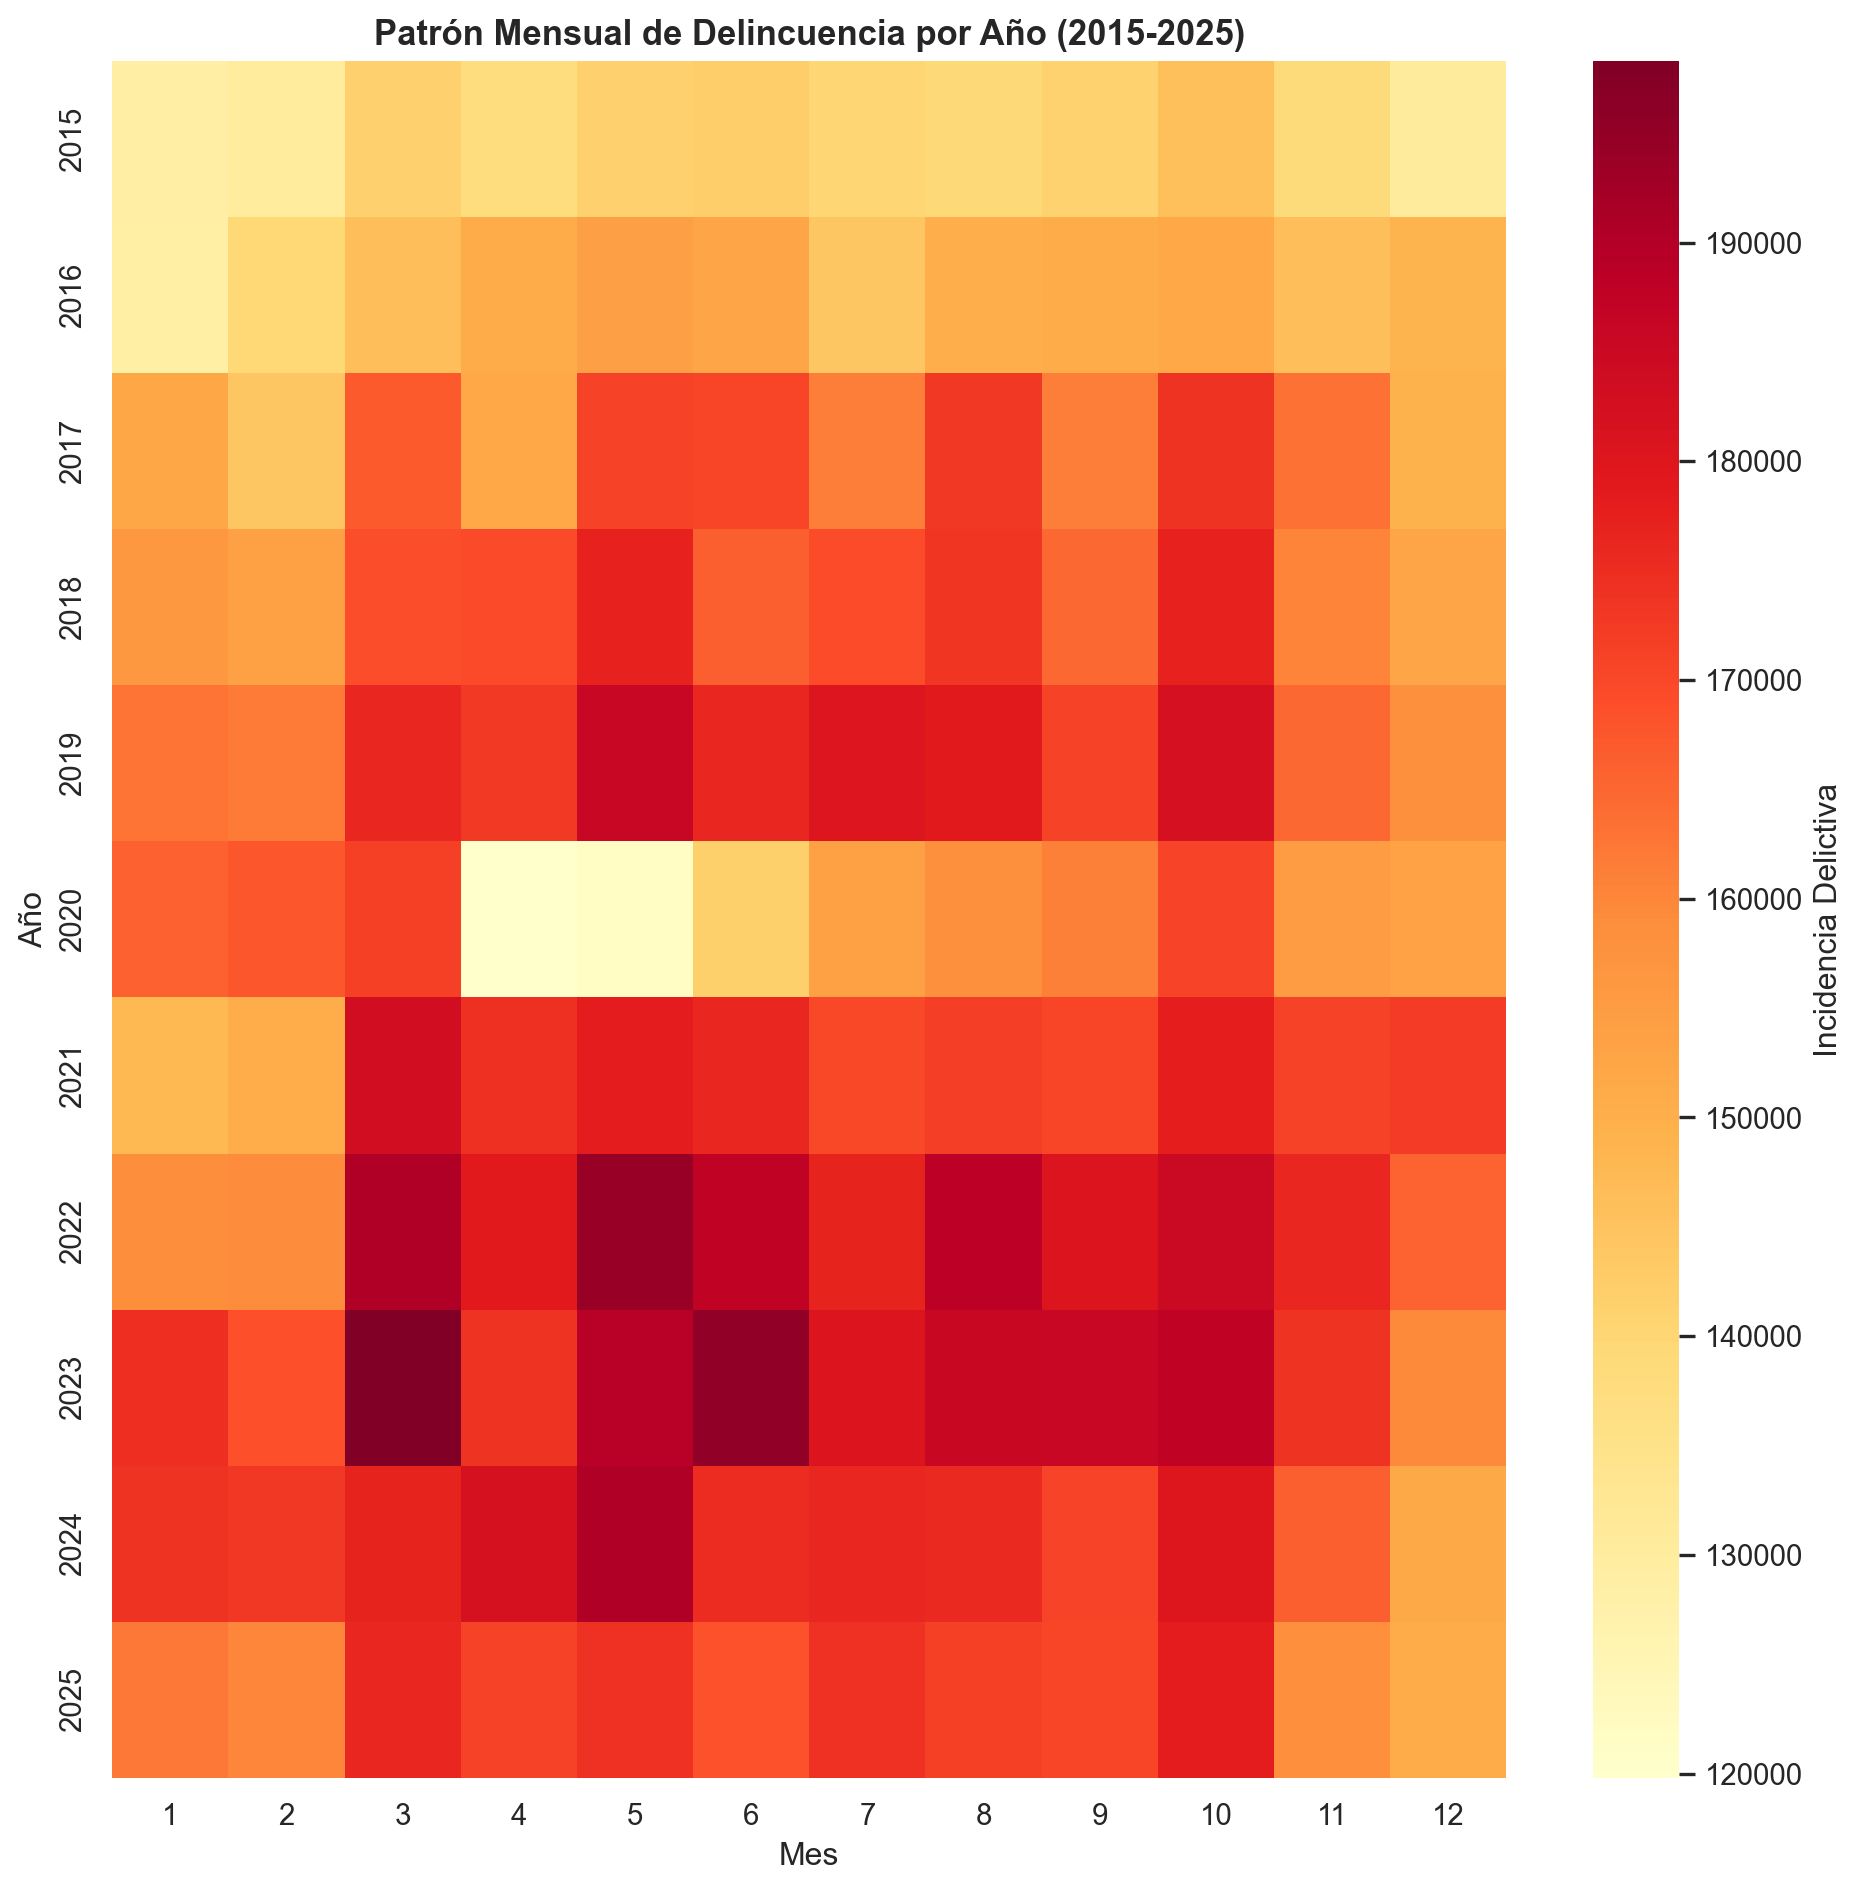
\includegraphics[width=0.8\textwidth]{imagenes/crime-by-month-output-1.png}
    \caption{Patrón Mensual de Delincuencia por Año en México (2015-2025)}
    \label{fig:crime-by-month}
\end{figure}

Vemos que en particular, de 2021 a 2025 el foco ha sido entre Marzo a Junio. Mientras que en años anteriores
habia sido de Mayo a Agosto (2015-2019). Lo que si es más fácil de notar con esto es que 2020 tiene los
valores más bajos de todos los años del conjunto, lo que puede deberse a que la incidencia delicitiva
realmente bajó durante ese periodo o que directamente no se reportó por completo.

\subsection{Detección de Outliers}

Para detectar outliers lo que haremos será ocupar IQR. Por lo anterior notamos que la incidencia delictiva
está fuertemente sesgada a la derecha por la CDMX y Edomex, ya que disparan los valores frente a estados
pequeños. El z-score asume normalidad y los propios extremos inflan media y desviación, así que ocupar ésta
medida reportaría resultados sesgados.

Para esto lo que haremos será ocupar la clase \texttt{OutlierDetector} que, como su nombre lo indica,
identificará los valores atípicos y luego usaremos su método flag() para aplicar ésta identificación a
un nuevo dataframe.

\begin{lstlisting}[language=Python, caption={Código para detectar outliers en la incidencia delictiva}, label={lst:outlier-detection}]
det = OutlierDetector(dataframe, columns=["incidencia_delictiva"])
det.summary()
\end{lstlisting}

\begin{table}[ht]
  \centering
  \caption{Resumen de Detección de Outliers}
  \scriptsize
  \resizebox{\textwidth}{!}{%
    \begin{tabular}{r r r l p{3.5cm} p{3cm} p{3cm} p{2.5cm} l l r l}
      \hline
      \textbf{idx} & \textbf{columna} & \textbf{Q1} & \textbf{Q3} & \textbf{IQR} & \textbf{Límite Inferior} & \textbf{Límite Superior} & \textbf{Número de Outliers} & \textbf{\% de Outliers} \\
      0 & incidencia\_delictiva & 413952 & 0.0 & 9968.0 & -39.0 & 65.0 & 63128 & 15.250077 \\
      \hline
    \end{tabular}%
  }
  \label{tab:outlier-summary}
\end{table}

Vemos que del total de registros, 63128 fueron identificados como outliers, lo que representa aproximadamente el 15.25\% del dataset. Esto es un
porcentaje considerable, pero dado el contexto de la delincuencia en México, es comprensible que existan registros con incidencias extremadamente
altas, especialmente en entidades como la CDMX y el EdoMex.

Sin embargo, es importante destacar que estos outliers no necesariamente representan errores en los datos, sino que reflejan la realidad de la
incidencia delictiva en ciertas regiones y periodos. Por lo tanto, en lugar de eliminar estos registros, se ha optado por marcarlos con una nueva
columna para su posterior análisis y consideración en cualquier modelado o interpretación de los datos. De esta manera, los datos se muestran como
sigue:

\begin{lstlisting}[language=Python, caption={Código para mostrar el dataset con la columna de outliers}, label={lst:dataset-con-outliers}]
det.flag()
\end{lstlisting}

\begin{table}[ht]
  \centering
  \caption{Muestra del dataset con columna de outliers}
  \scriptsize
  \resizebox{\textwidth}{!}{%
    \begin{tabular}{r r r l p{3.5cm} p{3cm} p{3cm} p{2.5cm} l l r l r}
      \hline
      \textbf{id} & \textbf{fecha} & \textbf{entidad} & \textbf{bien\_juridico\_afectado} & \textbf{tipo\_delito} & \textbf{subtipo\_delito} & \textbf{modalidad} & \textbf{incidencia\_delictiva} & \textbf{incidencia\_delectiva\_is\_outlier} \\
      \hline
      0 & 2015-04-01 & Aguascalientes & El patrimonio & Abuso de confianza & Abuso de confianza & Abuso de confianza & 22 & False \\
    1 & 2015-08-01 & Aguascalientes & El patrimonio & Abuso de confianza & Abuso de confianza & Abuso de confianza & 40 & False \\
    2 & 2015-12-01 & Aguascalientes & El patrimonio & Abuso de confianza & Abuso de confianza & Abuso de confianza & 26 & False \\
    3 & 2015-01-01 & Aguascalientes & El patrimonio & Abuso de confianza & Abuso de confianza & Abuso de confianza & 41 & False \\
    4 & 2015-02-01 & Aguascalientes & El patrimonio & Abuso de confianza & Abuso de confianza & Abuso de confianza & 33 & False \\
    \hline
    \end{tabular}%
  }
  \label{tab:dataset-outliers}
\end{table}